	\documentclass{if-beamer}
	\begin{document}
		
		\title[Campus Formoso do Araguaia]{Segurança da Informação}
		\subtitle{Aula 3 }
		\author{Gilmar Gomes do Nascimento}
		\institute[IFTO]{
			Instituto Federal do Tocantins\\
			Campus Formoso do Araguaia
		}
		\date{\today}
		\logo{
			
\includegraphics[scale=0.0085]{logo.jpg}
		}
		\subject{Security} % metadata
		
		\graphicspath{{figuras/}}
		%---------------------------------------------------------------------------------
		\begin{frame}
			\titlepage
		\end{frame}

		\begin{frame}{Definição de Proxy}
			Um proxy (em português `procurador', `representante') é um servidor (um sistema
			de computador ou uma aplicação) que age como um intermediário para requisições de
			clientes solicitando recursos de outros servidores

			\begin{figure}
				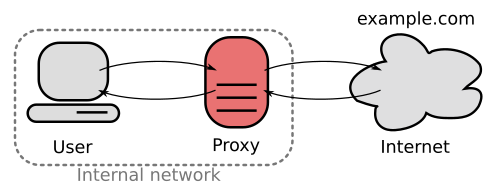
\includegraphics[scale=1]{proxy-example}
				% converter webp para png
			\end{figure}			
		\end{frame}

		\begin{frame}{Cliente}
			Um cliente conecta-se ao servidor proxy, solicitando algum serviço, como um arquivo, 
			conexão, página web ou outros recursos disponíveis de um servidor diferente, e o proxy
			avalia a solicitação como um meio de simplificar e controlar sua complexidade.			
		\end{frame}
		

		\begin{frame}[allowframebreaks]{Servidor de Proxy}
			 Os proxies foram inventados para adicionar estrutura e encapsulamento aos sistemas 
			 distribuídos. Esses servidores têm uma série de usos, como filtrar conteúdo,
			  providenciar anonimato, entre outros.
			\framebreak
			Um servidor proxy pode, opcionalmente, alterar a requisição do cliente ou a resposta 
			do servidor e, algumas vezes, pode disponibilizar este recurso mesmo sem se conectar 
			ao servidor especificado. Pode também atuar como um servidor que armazena dados em 
			forma de cache em redes de computadores. São instalados em máquinas com ligações 
			tipicamente superiores às dos clientes e com poder de armazenamento elevado.
			
			\framebreak

			\begin{figure}
				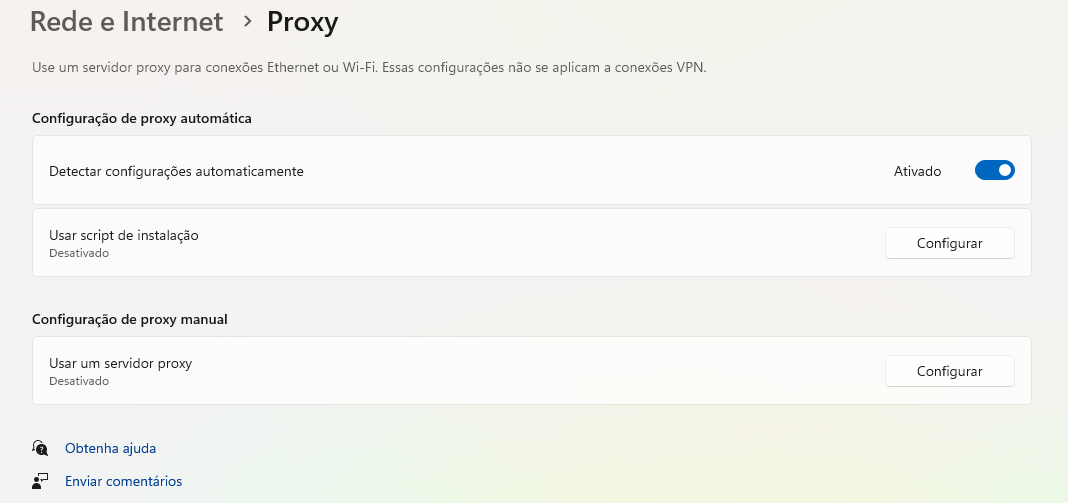
\includegraphics[scale=0.6]{settings-proxy}
			\end{figure}		
		\end{frame}
		
		\begin{frame}[allowframebreaks]{Squid Proxy Server}
			\begin{figure}
				
\includegraphics[scale=1]{squid-cache}
			\end{figure}
		\framebreak
		\begin{block}{Squid: Otimizando a entrega}
			Squid is a caching proxy for the Web supporting HTTP, HTTPS, FTP, and more. 
			It reduces bandwidth and improves response times by caching and reusing 
			frequently-requested web pages. Squid has extensive access controls and makes
			a great server accelerator. It runs on most available operating systems, including 
			Windows and is licensed under the GNU GPL.			
		\end{block}
		\framebreak

		\begin{block}{Making the most of your Internet Connection}
			Squid is used by hundreds of Internet Providers world-wide to provide their users
			 with the best possible web access. Squid optimises the data flow between client 
			 and server to improve performance and caches frequently-used content to save 
			 bandwidth. Squid can also route content requests to servers in a wide variety of 
			 ways to build cache server hierarchies which optimise network throughput.			
		\end{block}

		\framebreak

		\begin{block}{Website content acceleration and Distribution}
			Thousands of web-sites around the Internet use Squid to drastically increase their
			content delivery. Squid can reduce your server load and improve delivery speeds 
			to clients. Squid can also be used to deliver content from around the world -
			copying only the content being used, rather than inefficiently copying everything.
			Finally, Squid's advanced content routing configuration allows you to build content 
			clusters to route and load balance requests via a variety of web servers.			
		\end{block}			
		\end{frame}

		\begin{frame}{Hands-on}
			\begin{enumerate}
				\item Instale o Squid-cache na máquina virtual
				\item Mostre-me os status: funcionando, parado. 
				\item Configure para que não seja possível abrir nenhuma página com o domínio .bet na máquina virtual
			\end{enumerate}
			
		\end{frame}

		
		
		\begin{frame}[allowframebreaks]{Referências Bibliográficas}
			\bibitem{squid-cache}
	squid-cache.org \url{https://squid-cache.org}. Acessado em: 24 de agosto de 2026.

	\bibitem{Proxy-Wikipedia}
	PROXY. In: WIKIPÉDIA, a enciclopédia livre. Flórida: Wikimedia Foundation, 2024. 
	Disponível em: \url{https://pt.wikipedia.org/w/index.php?title=Proxy&oldid=68693766}. Acesso em: 24 agosto. 2026.

	\bibitem{ibm}
	IBM. (2025). Tivoli Application Dependency Discovery Manager. \url{https://www.ibm.com/docs/pt-br/taddm/7.3.0?topic=problems-synchronization-server}. Acessado em: 6 de agosto de 2026.

	\bibitem{cisco}
	Cisco. (2025). Use as práticas recomendadas para o Network Time Protocol. \url{https://www.cisco.com/c/pt_br/support/docs/availability/high-availability/19643-ntpm.html}. Acessado em: 6 de agosto de 2026.

	\bibitem{suse}
	SUSE. (2026). Sincronizando o horário por meio de NTP/NTS. \url{https://documentation.suse.com/pt-br/sle-micro/6.1/html/Micro-ntp-time-synchronization/index.html}. Acessado em: 6 de agosto de 2026.

	\bibitem{Moreiras2021}
	Moreiras, Antonio Marcos. (2021). NTP e NTS de Forma Correta e Segura, Sincronismo de Tempo na Internet. Nic.br. \url{https://bibliotecadigital.acervo.nic.br/server/api/core/bitstreams/129d1169-25b5-49ce-b015-28ffadc440da/content}. Acessado em: 6 de agosto de 2026.
		\end{frame}	
		
	\end{document}
